% !TEX root =  ../main.tex

\begin{figure*}[t]
	\centering
	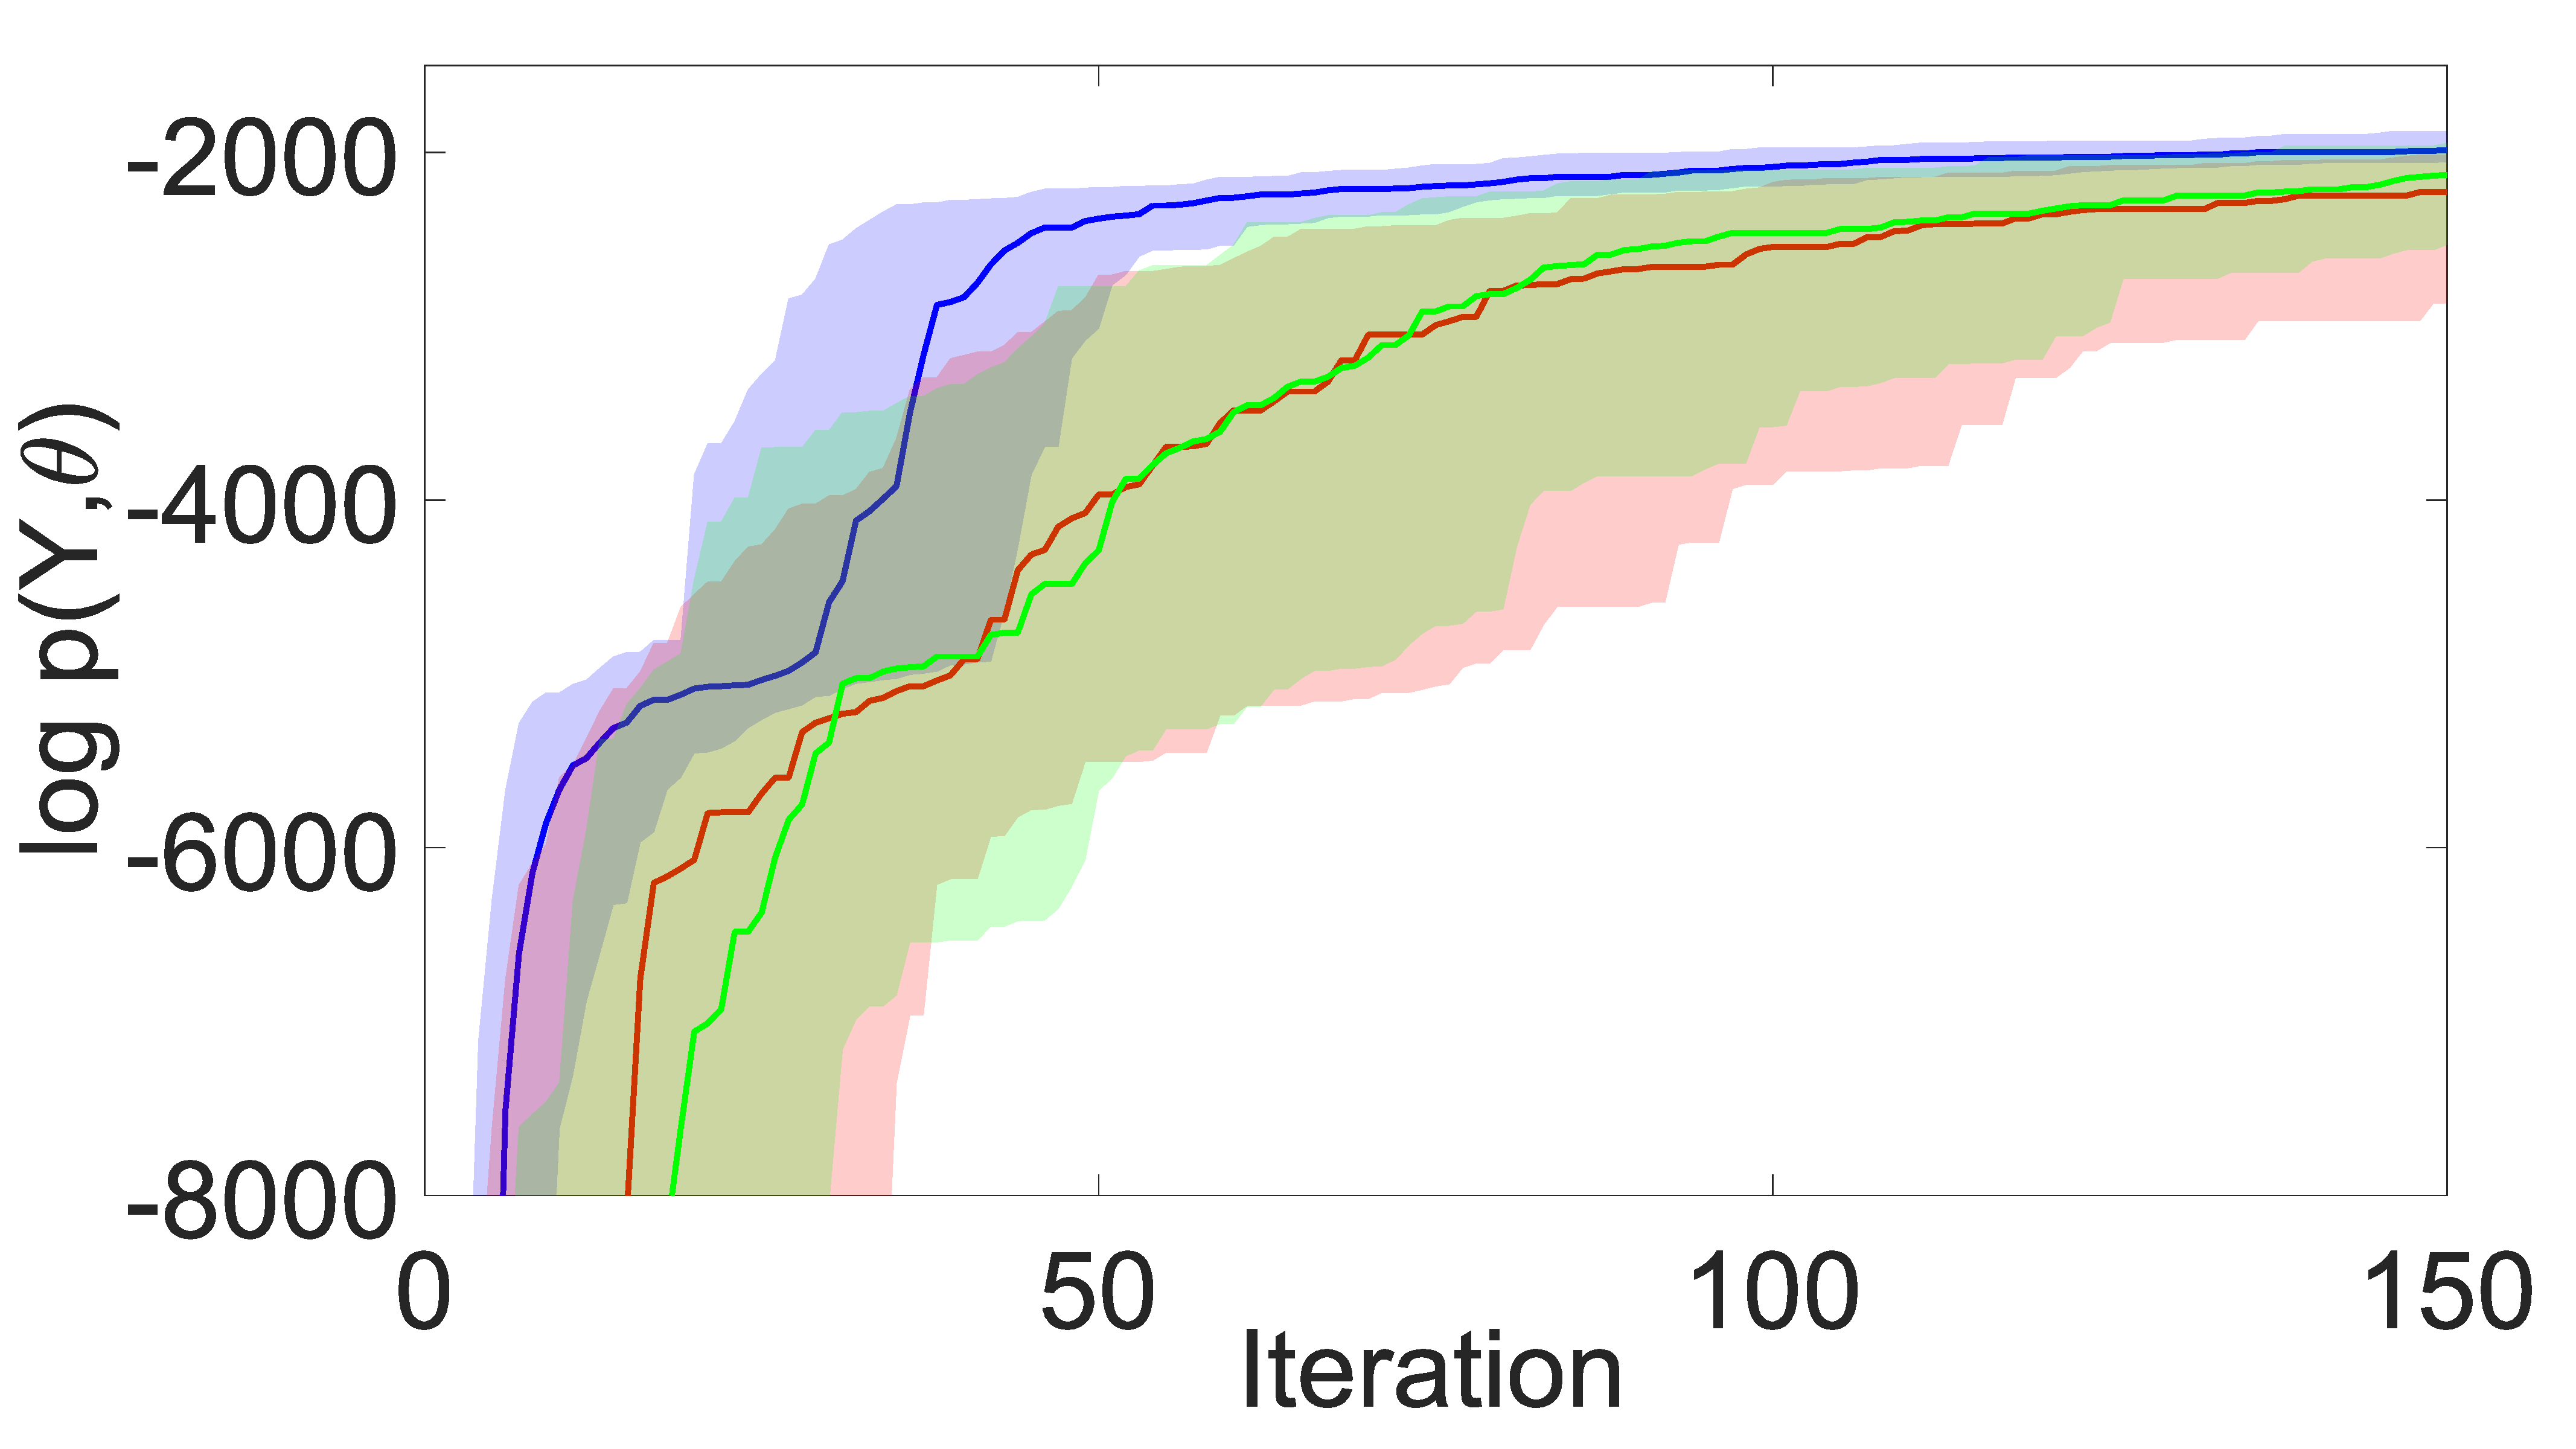
\includegraphics[width=2.72in]{hmm/hmm_ML}
	~~~~~~
	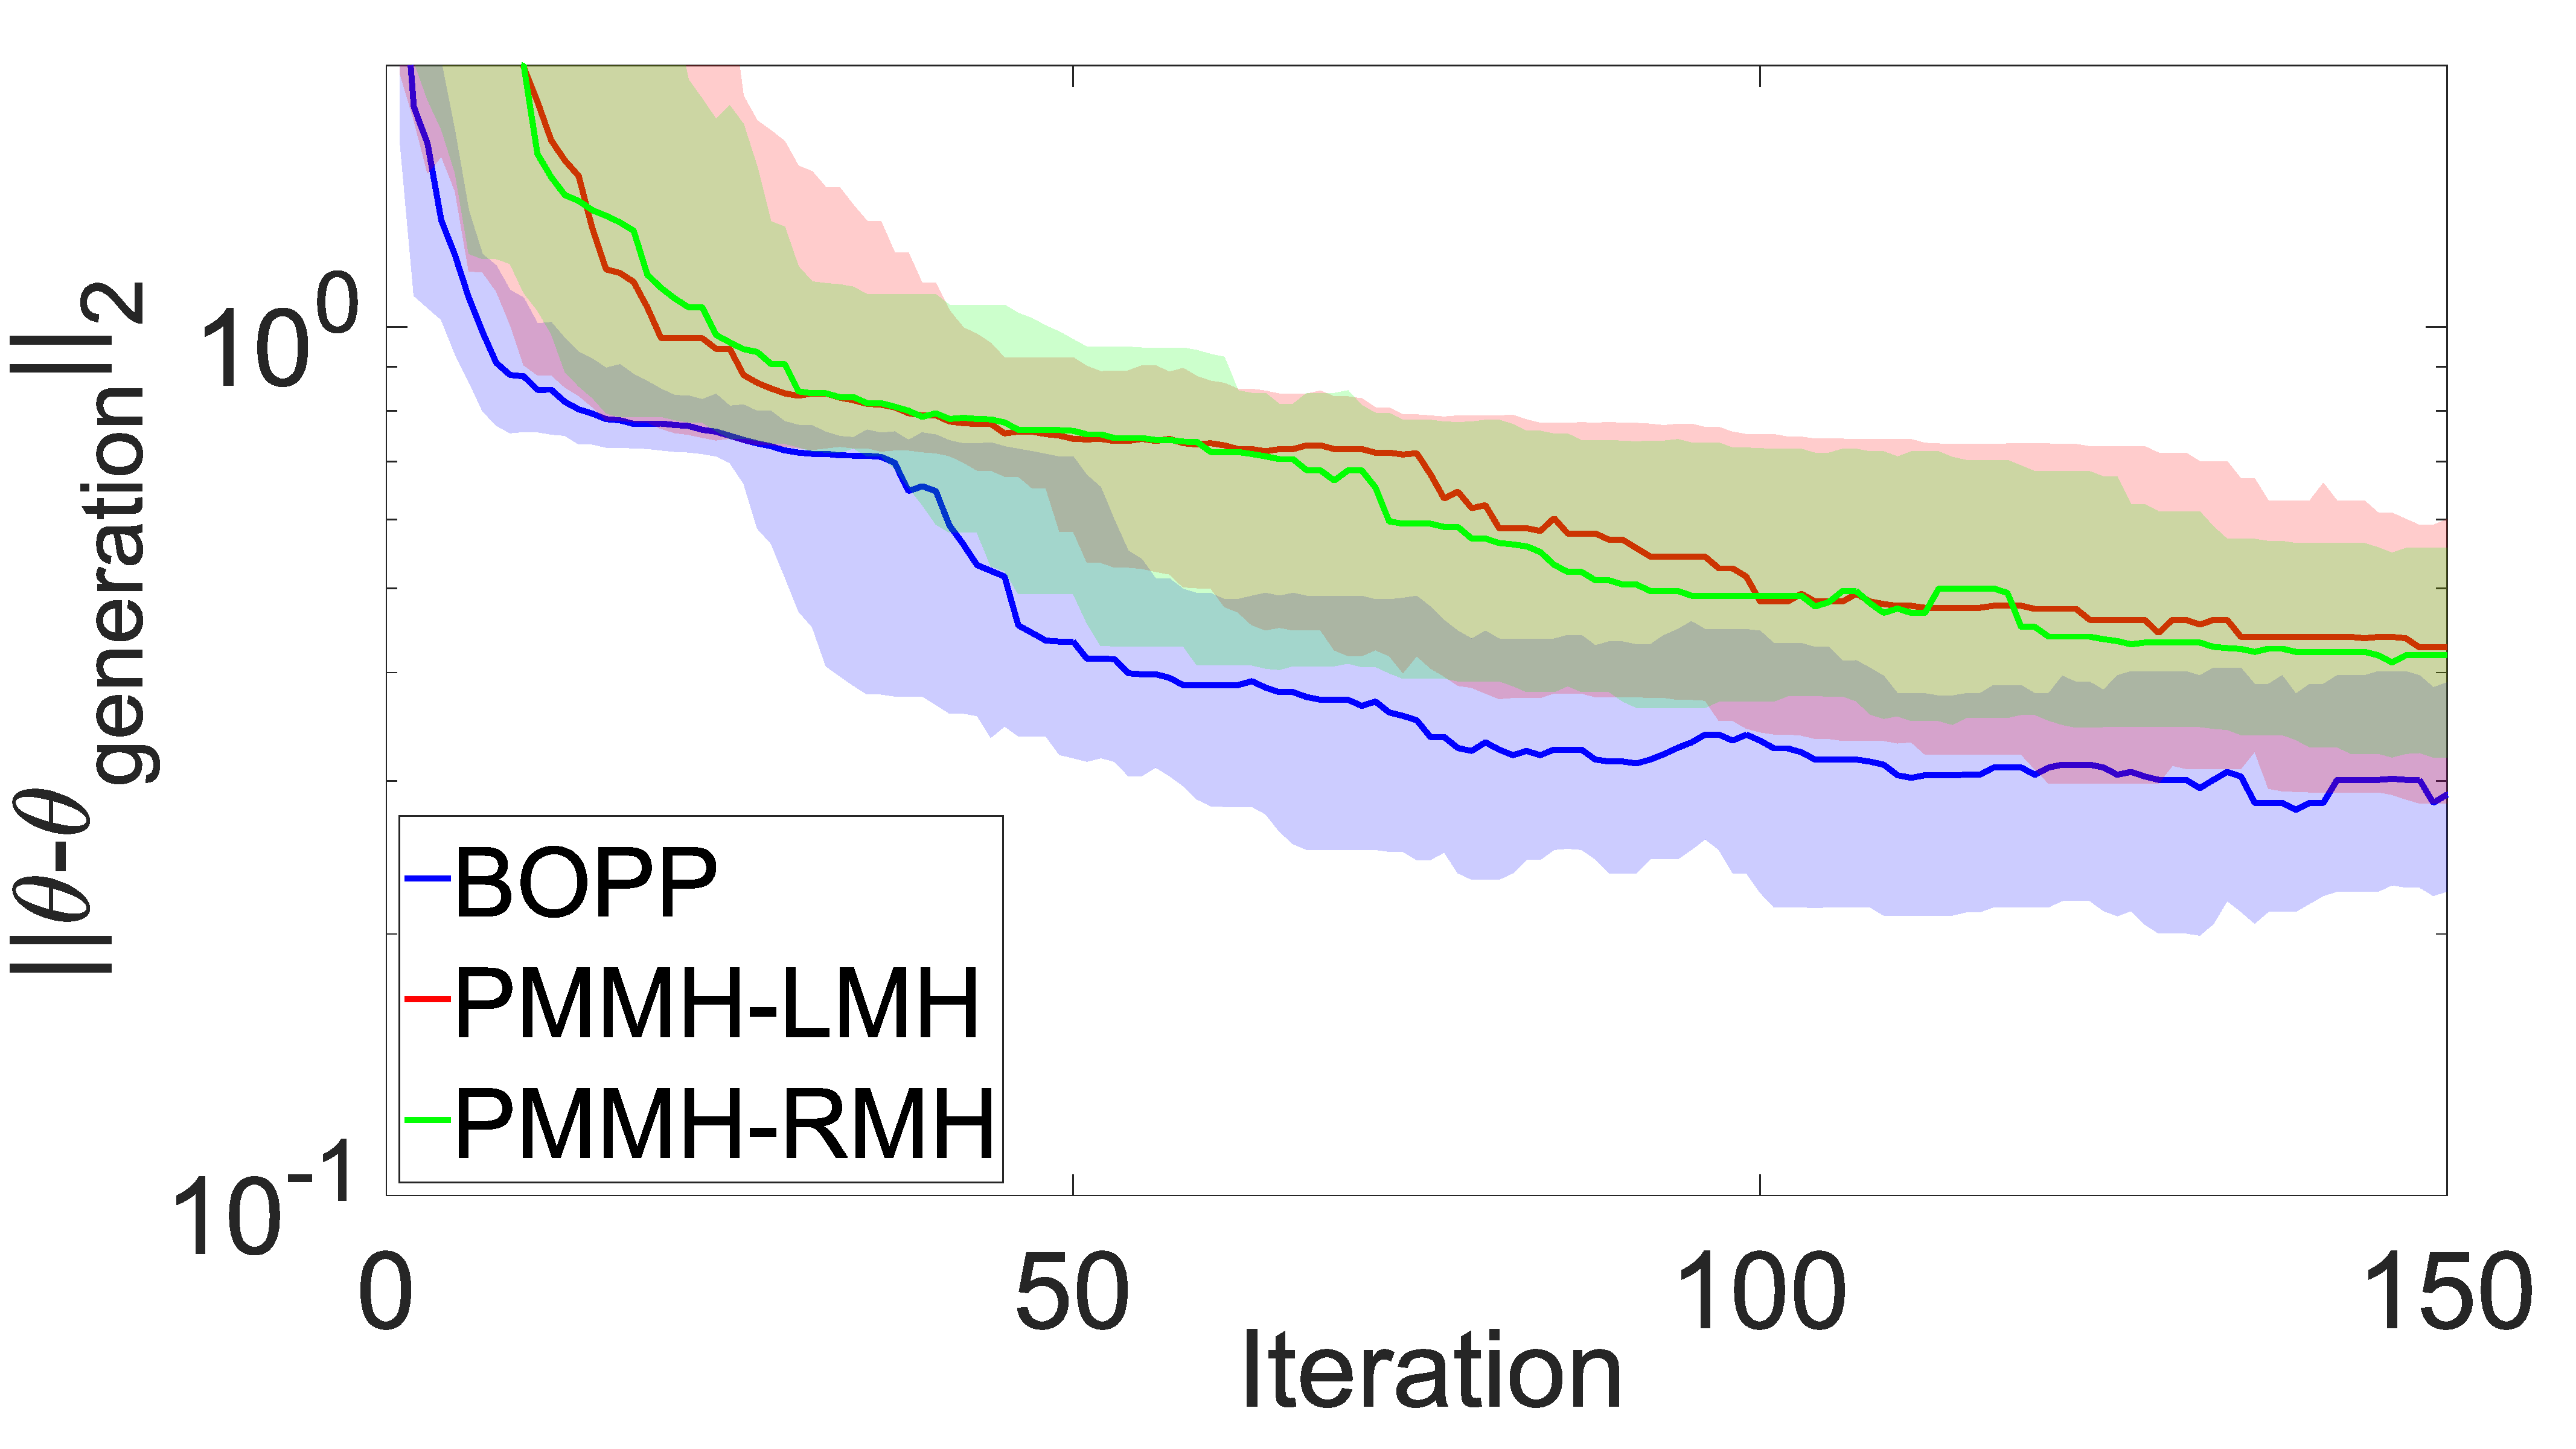
\includegraphics[width=2.72in]{hmm/hmm_distance}
	\caption{Convergence for HMM in terms of the cumulative best $\log p\left(Y,\theta\right)$ (\emph{left}) and distance to the ``true" $\theta$ used in generating the data (\emph{right}). Solid line shows median over 100 runs, whilst the shaded region the 25/75\% quantiles.  Note that for the distance to true $\theta$ was calculated by selecting the three states (out of the 5 generated) that were closest to the true parameters.  \label{fig:hmm}}
\end{figure*}

We finish by considering a hidden Markov model (HMM) with an unknown number of discrete possible states.  
This example demonstrates how BOPP can still be applied to models which conceptually have an 
unknown number of target variables, by generating all possible variables that might be needed, 
but then leaving some variables unused for some execution traces.  This avoids problems 
of varying reference measures so that the MMAP problem is well defined  and provides a 
function with a fixed number of inputs as required by the BO scheme.  From the BO 
perspective, the target function is simply constant for variations in an unused variable.

Our model places a uniform prior on the number of states $K \sim \textsc{Discrete}\{1,2,3,4,5\}$.
Each emission distribution corresponds to a Gaussian with unknown mean (which we wish to
optimize) and known variance.  
We marginalize over the transition distribution parameters and the HMM latent states.  
Rather than constructing a model where the emission distribution
parameters only exist conditioned on the value of $K$, we generate variables for all $5$ emission
distributions that might be required, with only the first $K$ actually then used.  
A synthetic dataset was generated using $K=3$ and $T=1000$ observations.  Results of running BOPP are given
in Figure~\ref{fig:hmm}, again showing that BOPP outperforms these PMMH alternatives.  See~\cite{rainforth2017boppArxiv}
for further details.